\documentclass{article}

\usepackage[utf8]{inputenc}
\usepackage[frenchb]{babel}
\usepackage[T1]{fontenc}
\usepackage{graphicx}
\usepackage{amsmath,amsfonts,amssymb}
\usepackage{pgfplots}
\usepackage{lscape}
\usepackage{braket}
\usepackage{multirow}
\usepackage{hyperref}
\usepackage{listings}
\usepackage{color}
\usepackage{float}
\usepackage{ulem}
\usepackage{framed}
\definecolor{lightgray}{rgb}{.9,.9,.9}
\definecolor{darkgray}{rgb}{.4,.4,.4}
\definecolor{purple}{rgb}{0.65, 0.12, 0.82}

\newcommand{\Sha}{\textls[0]{III}}

\lstdefinelanguage{JavaScript}{
  keywords={include, mesh, physical, group, function, jacobian, integration, constraint, functionspace, formulation, resolution, postprocessing, postoperation, name, case, operation},
  keywordstyle=\color{blue}\bfseries,
  ndkeywords={class, export, boolean, throw, implements, import, this},
  ndkeywordstyle=\color{darkgray}\bfseries,
  identifierstyle=\color{black},
  sensitive=false,
  comment=[l]{//},
  morecomment=[s]{/*}{*/},
  commentstyle=\color{purple}\ttfamily,
  stringstyle=\color{red}\ttfamily,
  morestring=[b]',
  morestring=[b]"
}

\lstset{
   language=JavaScript,
   extendedchars=true,
   basicstyle=\footnotesize\ttfamily,
   showstringspaces=false,
   showspaces=false,
   numbers=left,
   numberstyle=\footnotesize,
   numbersep=9pt,
   tabsize=2,
   breaklines=true,
   showtabs=false,
   captionpos=b
}

\usepackage[europeanvoltages, europeancurrents, europeanresistors, americaninductors]{circuitikz}

\usepackage{fancyhdr}
\usepackage[headheight = 2cm,bottom=3.5cm]{geometry}
\pagestyle{fancy}
\renewcommand{\headrulewidth}{1pt}
\fancyhead[L]{
\includegraphics[height=1.5cm]{assets/logocs.png}} 
\fancyhead[C]{\textsc{Performance analysis of a batched\\ parallel reduction using CUDA\\}}
\fancyhead[R]{
\includegraphics[height=1.5cm]{assets/soprasteria.png}}
\renewcommand{\footrulewidth}{1pt}
\fancyfoot[C]{} 
\fancyfoot[L]{\href{https://drive.google.com/open?id=1ETwTI8ptyoaDpvvjFe6wB5ziKXfQL0BL}{Baptiste Legouix}}


\begin{document}
\title{\vspace{-70pt}\textsc{CS Group} \\
\vspace{10pt}\hspace*{-25pt}\begin{tabular}{cc}
\multirow{4}{*}{
\begin{minipage}{0.20\textwidth}\vspace{15pt}
\includegraphics[scale=0.53]{assets/biglogocs.png}\end{minipage}} & \rule{0.60\linewidth}{0.5pt}\vspace{10pt} \\ & Performance analysis of a batched\\ & parallel reduction using CUDA\\ & \rule{0.60\linewidth}{2pt}
\end{tabular}}
\author{\href{https://drive.google.com/open?id=1ETwTI8ptyoaDpvvjFe6wB5ziKXfQL0BL}{Baptiste Legouix}}
%\date{\today\\[30pt] \huge \ccbynd}
\date{\today}

\clearpage
\maketitle
\thispagestyle{empty}

\vspace{0pt}
\begin{center}
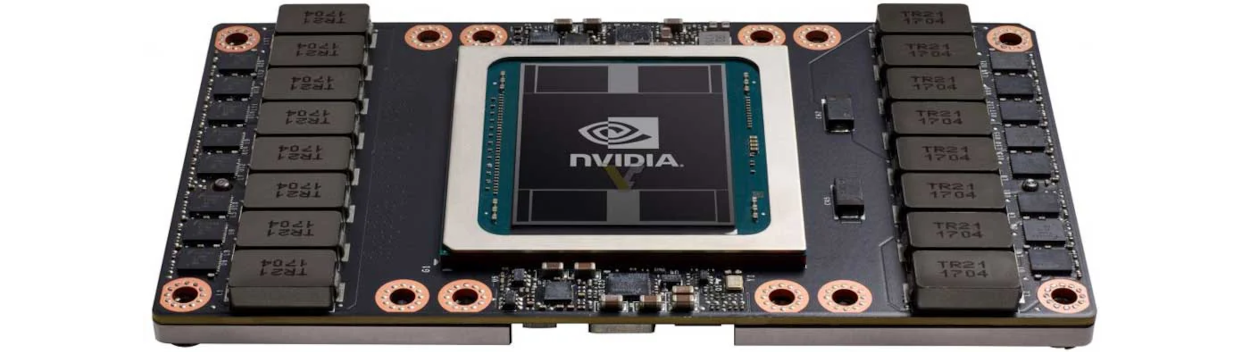
\includegraphics[width=0.7\textwidth]{assets/cover.png}
\end{center}
\vspace{0pt}

\tableofcontents

\vspace{30pt}

\subsection*{Abstract}

placeholder

\newpage

\setcounter{page}{1}
\fancyfoot[R]{\thepage}

\section{GPU performance programming}

% \subsection*{Introduction}

\subsection{GPU Architecture}

\textit{Graphical Processor Units} differentiate themselves from CPU by relying on the SIMT (Single-Instruction, Multiple Threads) execution model. It means an instruction in a CUDA computing kernel has to be executed by all the \textit{threads} forming a \textit{warp}, synchronously.

The hardware architecture of the GPU is as follow:

\begin{figure}[H]
\begin{center}
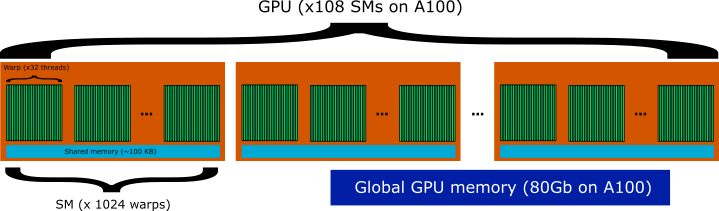
\includegraphics[width=\textwidth]{assets/gpu_arch.png}
\end{center}
\label{fig:gpu_arch}
\end{figure}

If threads inside a warp are automatically synchronized due to the SIMT model (an instruction has to be executed by all the threads within the warp before executing the next one), warps within a \textit{Stream Multiprocessor} or SMs within the GPU are running concurrently but not synchronously. It means warps and SM have to be synchronized using dedicated CUDA instruction to prevent race conditions.

Note: if threads within a warp are running synchronously, the \textit{ordering} of the execution is undetermined (we do not know which thread will be the first to finish the execution of a single instruction).

Note: since CUDA 9, the SIMT model has been slightly relaxed which can lead to subtle desynchronizations within a warp, which justify the need for the \textit{\_\_syncwarp()} CUDA function.

\subsection{CUDA programming model}

CUDA is the native language provided by Nvidia (chip manufacturer) to program for GPU. It relies on \textit{CUDA kernels} which contain the code to be executed on the GPU. 

The calls to launch CUDA kernels are parametrized with two compile-time integers: the \textit{grid size} and the \emph{block size}. Those two numbers correspond respectively to the number of SM and the number of threads per SM to execute the CUDA kernel. If the block size is not a multiple of the warp size (which is 32 in all current architectures), the compiler will automatically mask off exceeding threads within the last warp. Actually, CUDA allows to configure kernels with pairs or triplet of integers to conveniently run through multidimensional arrays (until 3D), but this is internally flattened to a 1D map so we will discuss only the 1D grid and block sizes.

\subsection{Performance guidelines}

There are plently of ways to improve the performance of a code running on GPU, and Nvidia provides dedicated tools to measure and analyse the differents processes that may impact the performance. We list here the main topics we are interested in this mini-project:

\begin{itemize}
	\item Get the highest possible GPU occupancy (as much threads as possible must be active simultaneously).
	\item Using memory \textit{to the nearest} of the thread (avoid the allocation of buffers in the global memory if shared memory\cite{cudasharedmemory} or registers can be used).
	\item Order correctly the data stored in the global memory to read and write it efficiently (coalescent accesses).
\end{itemize}

\section{Batched reduction problem}

\subsection{Presentation}

A batched reduction is a mathematical operation which aims to compute from a matrix $A$ the vector $B$ containing the sums:

\[
B_i = \sum_{j<N} = A_{ij}
\]

From the physical point-of-view, this operation is involved in the numerical computation of integrals along a $1D$ dimension in an $ND$ space:

\[
b(y, z, ...) = \int a(x, y, z, ...)\; dx
\]

The index $j$ corresponds to the discretization of the \textit{dimension of interest} (ie. $x$) while the index $i$ corresponds to the other dimensions (ie. $y, z, ...$).

The interest of the study of this numerical problem from the performance point-of-view is that this is a very simple example of problem which is manifestly parallelizable but may require communication between threads depending on the algorithm chosen for its resolution.

\subsection{Algorithms}

\subsubsection{Sequential embarassing parallelization}

An \textit{embarassingly parallel} problem is composed of subproblems which are all independent one-to-the-others. It is then very simple to parallelize as no communication between threads is required. All buffers can be written in the thread-local registers.

The batched reduction is embarassingly parallel along the batch index $i$. The following CUDA kernel can thus be written to obtain an implementation where each thread computes a unitary reduction using a sequential \textit{for} loop:

\begin{lstlisting}[language=C++]
template <std::size_t M, std::size_t N, class Layout>
__global__ void sequential_kernel(
    cuda::std::mdspan<double, cuda::std::extents<std::size_t, M>> B,
    cuda::std::mdspan<double, cuda::std::extents<std::size_t, M, N>, Layout> A) {
  std::size_t i = blockIdx.x * blockDim.x + threadIdx.x;

  double sum = 0;

  for (std::size_t j = 0; j < N; ++j) {
    sum += A(i, j);
  }

  B(i) = sum;
}
\end{lstlisting}

\subsubsection{\textit{cooperative\_groups::reduce}-based parallelization}

The problem of sequential algorithm is that a small value for $M$ should lead to low occupancy of the GPU threads. We should thus explore more sophisticated algorithm which parallelize the unitary reductions themselves.

Such algorithms can be directly written in CUDA. This is though not something we discuss in this document, because we expect standard implementations provided by Nvidia to be already optimized and thus produce the best possible performances if correctly used. We begin by relying on the \textit{cooperative\_groups::reduce} method, which is the lowest-level function dedicated to reduction provided in CUDA.

\begin{lstlisting}[language=C++]
template <std::size_t M, std::size_t N, class Layout>
__global__ void cooperative_groups_kernel(
    cuda::std::mdspan<double, cuda::std::extents<std::size_t, M>> B,
    cuda::std::mdspan<double, cuda::std::extents<std::size_t, M, N>, Layout> A) {
  std::size_t i = blockIdx.x;
  std::size_t j = threadIdx.x;

  double val = A(i, j);

  // Perform reduction within the block
  cooperative_groups::thread_block_tile<32> tile32 =
      cooperative_groups::tiled_partition<32>(
          cooperative_groups::this_thread_block());
  double partial_sum = cooperative_groups::reduce(
      tile32, val, cooperative_groups::plus<double>());

  __shared__ double partial_sums[(N + 31) / 32];

  // Thread 0 of each warp writes result to partial_sums
  if (tile32.thread_rank() == 0) {
    partial_sums[tile32.meta_group_rank()] = partial_sum;
  }

  cooperative_groups::this_thread_block().sync();

  // Thread 0 of warp 0 aggregates the partial sums
  if (cooperative_groups::this_thread_block().thread_rank() == 0) {
    double sum = 0.0;
    for (std::size_t k = 0; k < (N + 31) / 32; ++k) {
      sum += partial_sums[k];
    }
    B(i) = sum;
  }
}
\end{lstlisting}

The strategy is the following: we declare \textit{tile32} to represent a warp, and we rely on \textit{cooperative\_groups::reduce} to perform the reduction within each warp, leading to partial sums of $32$ elements stored in the shared memory. We then use the very first thread of the block (indexed by $j=0$) to finally perform the sum of the partial sums sequentially and write it in the global memory.

\subsubsection{\textit{CUB}-based parallelization}

\textit{CUB} is a Nvidia library which provides higher-level function compared to CUDA. It contains in particular thread, warp, block and device-level functions dedicated to reduction:

\begin{itemize}
	\item The thread-level reduction function corresponds exactly to the implementation proposed in the \textit{Sequential embarassing parallelization section}.
	\item The warp-level reduction corresponds probably to the \textit{cooperative\_groups::reduce} function when applied on a tile representing a warp.
	\item The block-level reduction corresponds probably to our \textit{cooperative\_groups\_kernel} function presented above.
	\item The device-level reduction is called from CPU but implements a non-batched reduction, thus does not suit our needs.
\end{itemize}

The measurements exhibited very similar performance between the \textit{cooperative\_groups\_kernel} from the precedent section, and the block-level \textit{CUB} reduction below using the \textit{BLOCK\_REDUCE\_WARP\_REDUCTIONS} algorithm. We thus won't report the measurements with \textit{cooperative\_groups\_kernel} because I suspect both methods to be perfectly equivalent.

\begin{lstlisting}[language=C++]
template <cub::BlockReduceAlgorithm Algorithm, std::size_t M, std::size_t N,
          class Layout>
__global__ void cub_block_reduction_kernel(
    cuda::std::mdspan<double, cuda::std::extents<std::size_t, M>> B,
    cuda::std::mdspan<double, cuda::std::extents<std::size_t, M, N>, Layout> A) {
  std::size_t i = blockIdx.x;
  std::size_t j = threadIdx.x;

  double val;

  val = A(i, j);

  __shared__ typename cub::BlockReduce<double, N, Algorithm>::TempStorage temp_storage;

  double block_sum =
      cub::BlockReduce<double, N, Algorithm>(temp_storage).Sum(val);

  if (j == 0) {
    B(i) = block_sum;
  }
}
\end{lstlisting}

Two algorithms have been tested. Please refer on the \textit{CUB} documentation for details:

\begin{itemize}
\item BLOCK\_REDUCE\_WARP\_REDUCTIONS
\item BLOCK\_REDUCE\_RAKING\_COMMUTATIVE\_ONLY 
\end{itemize}

\subsection{Memory layout for $A$ in the global memory}

$A$ being a matrix, there are several ways to store it in the global memory. We test four layouts:

\begin{itemize}
	\item \textit{Right} layout: the $j$ indexing is contiguous.
	\item \textit{Left} layout: the $i$ indexing is contiguous.
	\item \textit{RightStride} layout: the $j$ indexing is contiguous but \textit{by blocks of 32 elements}. The idea is to fit the size of a warp.
	\item \textit{LeftStride} layout: the $i$ indexing is contiguous but \textit{by blocks of 32 elements}. The idea is to fit the size of a warp.
\end{itemize}

\section{Performance results}

We report the first evaluation of performance of the several approaches presented above. As mentioned precedently, the measurements with \textit{cooperative\_groups\_kernel} are not reported because I suspect it to be perfectly equivalent to the \textit{BLOCK\_REDUCE\_WARP\_REDUCTIONS} algorithm.

The tests are performed on a $A100$ GPU. Every layouts are tested for every method. We have three reference size tests:

\begin{itemize}
	\item $N = 1024$ and $M=32$ which is a small case where each warp can perform a complete unitary reduction using the \textit{CUB} block-reduction methods.
	\item $N = 1024$ and $M=1024$ which is a case where each SM can perform a complete unitary reduction using the \textit{CUB} block-reduction methods.
	\item $N = 1024$ and $M=1024$ which is a case big enough to fill the GPU even using the sequential embarassingly-parallel method.
\end{itemize}

\newpage
\nocite{*}
\bibliographystyle{unsrt}
\bibliography{biblio}

\end{document}
